\documentclass[letterpaper,landscape,9pt,fleqn]{extarticle}
\usepackage[document]{ragged2e}
\usepackage[utf8]{inputenc}
\usepackage[T1]{fontenc}
\usepackage{graphicx}
\usepackage{xcolor}
\usepackage{tikz}
\usepackage{url}
\usepackage{qrcode}
\usetikzlibrary{shapes.geometric}
\usetikzlibrary{calc}
\usepackage{array}   % for \newcolumntype macro
%\usepackage{fourier}
\usepackage{graphicx,nicefrac}
\usepackage{isomath,upgreek,xcolor,comment,fourier}
\usepackage{pdfpages}
\usepackage{tkz-euclide}
\usepackage{enumitem}
%\usetkzobj{all}
\pagestyle{empty}
\usepackage[final]{microtype}
\usepackage[american]{babel}

\usepackage{amstext} % for \text macro
\usepackage{array}   % for \newcolumntype macro
\newcolumntype{L}{>{$}l<{$}} % math-mode version of "l" column type

\newcommand{\dom}{\mathrm{dom}} 
\newcommand{\range}{\mathrm{range}} 
\newcommand{\zero}{\mathrm{zero}} 
\newcommand{\reals}{\mathbf{R}} 
\newcommand{\integers}{\mathbf{Z}} 
\newcommand{\ssep}{\mid}
\newcommand{\arcsec}{\mathrm{arcsec}}
\newcommand{\arccsc}{\mathrm{arccsc}}
\newcommand{\arccot}{\mathrm{arccot}}

\usepackage{amsmath,amssymb,textcomp}
\everymath{\displaystyle}
\usepackage{tgheros}
\usepackage{multicol}
\setlength{\columnseprule}{0pt}
\setlength{\columnsep}{15pt}


\usepackage{geometry}
\geometry{letterpaper,left=5mm,right=5mm,top=5mm,bottom=5mm}

%\linespread{1}



% custom section
\usepackage[explicit]{titlesec}
\newcommand*\sectionlabel{}
\titleformat{\section}
  {\gdef\sectionlabel{}
   \normalfont\sffamily\Large\bfseries\scshape}
  {\gdef\sectionlabel{\thesection\ }}{0pt}
  {
\noindent
\begin{tikzpicture}
\node[rectangle,rounded corners=3pt,inner sep=4pt,fill=blue!50!black,text width= 0.95\columnwidth] {\color{white}\sectionlabel#1};
\end{tikzpicture}
  }

\raggedbottom 
%\allowdisplaybreaks
\usepackage{tikz-3dplot}
\begin{document}

\setlength{\parskip}{-6mm}
\begin{multicols*}{4}
\section*{Named Sets}
\begin{minipage}[c]{0.25\textwidth}
\begin{tabular}{|L | L |} \hline 
   \text{empty set} & \varnothing \\ 
   \text{real numbers} & \reals \\
   \text{ordered pairs }  & \reals^2 \\
   \text{integers} & \integers \\
  \text{positive integers} & \integers_{>0} \\ 
  \text{positive  real  numbers} & \reals_{>0} \\
  \hline
  \end{tabular}
  \end{minipage}
  \vspace{0.1in}
\section*{Exponents}
\begin{minipage}[c]{0.25\textwidth}
  For \(a,b \in \reals_{>0},  x \in \reals\), and \(m,n \in \reals\),
  \begin{align*}
  &a^0 = 1,  &0^a = 0\\
  &1^x = 1,   &a^n a^m = a^{n+m}  \\
  &\nicefrac{a^n}{a^m} = a^{n-m}, &(a^n)^m = a^{n \cdot m} \\
  &a^{-m} = \nicefrac{1}{a^m},   &\left(\nicefrac{a}{b}\right)^m = \nicefrac{a^m}{b^m} \\
  &\sqrt{x^2} = |x| &\phantom{xxx}
\end{align*}
 \end{minipage}
 \vspace{0.1in}
\section*{Trigonometric Identities}
%\vspace{-0.25in}
\begin{minipage}[c]{0.25\textwidth}
  We define $\dom(\arccot) = (0,\uppi)$.
\begin{align*}
  &\left(\cos(x)\right)^2 + \left(\sin(x)\right)^2 = 1 \\
  &2 \left(\cos(x)\right)^2 =  1 + \cos(2 x) \\
  &2 \left(\sin(x)\right)^2 = 1 - \cos(2 x) \\
  & \left(\cos (x)\right)^2 - \left(\sin (x) \right)^2 = \cos(2x) \\
   &\sin\left(x +  y\right) =\sin (x) \cos (y) + \cos (x) \sin (y) \\
  &\cos\left(x+y\right)=\cos (x) \cos (y) - \sin (x) \sin (y)    \\
  &\arccot(x) = \nicefrac{\uppi}{2} - \arctan(x) \\
  &\arccsc(x) = \arcsin \left (\nicefrac{1}{x} \right ) \\
  &\arcsec(x) = \arccos \left(\nicefrac{1}{x} \right) \\
  & \arcsin (x) + \arccos (x) = \nicefrac{\uppi}{2} \\
    & \arcsec (x) + \arccsc (x) = \nicefrac{\uppi}{2}
  \end{align*}
\end{minipage}
\vspace{0.1in}
\section*{Hyperbolic Functions}
%\vspace{-0.35in}
\begin{align*}
  &2 \cosh(x) = \exp(x) + \exp(-x) \\
  &2 \sinh(x) = \exp(x) - \exp(-x) \\
  & \tanh(x) = \nicefrac{\sinh(x)}{\cosh(x)}\\
  &\cosh(x)^2 - \sinh(x)^2 = 1
\end{align*}
\vspace{0.1in}
  \section*{Logarithms}
 % \vspace{-0.15in}
      \begin{equation*}
    \log_a(x) = \frac{\ln(x)}{\ln(a)}
       \end{equation*}
\newcolumn

\section*{Derivatives}
\textbf{Specific cases} \\
\begin{tabular}{| L | L | L|}
\hline
F(x)  & F^\prime(x) \\ \hline 
\cos(x)  &  -\sin(x)    \\
\sin(x)  &  \cos(x)   \\
\tan(x)  & \sec(x)^2  \\  
\sec(x)  &  \sec(x) \tan(x) \\
\csc(x)  & -\cot(x) \csc(x) \\
\cot(x)  &  -\csc(x)^2 \\
\arccos(x)  & -\nicefrac{1}{\sqrt{1-{{x}^{2}}}}   \\
\arcsin(x)  & \nicefrac{1}{\sqrt{1-{{x}^{2}}}}\\
\arctan(x) &  \nicefrac{1}{\big (x^2+1 \big)}  \\  
%\arcsec(x) & \nicefrac{1}{ \big (\sqrt{{{x}^{2}}-1}\, \left| x\right| \big )} \\
%\arccsc(x)   & -\nicefrac{1}{ \big (\sqrt{{{x}^{2}}-1}\, \left| x\right| \big ) } \\
%\arccot(x)   & -\nicefrac{1}{ \big (x^2+1 \big )} \\ 
\cosh(x)  &  \sinh(x)    \\
\sinh(x)  &  \cosh(x)   \\
\tanh(x)  & 1/\cosh(x)^2  \\ 
\mathrm{arccosh}(x)  & \nicefrac{1}{\sqrt{x^2-1}}   \\
\mathrm{arcsinh}(x)  & \nicefrac{1}{\sqrt{1+{{x}^{2}}}}\\
\mathrm{arctanh}(x) &  \nicefrac{1}{{(1-{x}^{2}})}  \\
\exp(x) & \exp(x)    \\
\ln(x)  & 1/x    \\ \hline
%\log_a(x) & \nicefrac{1}{x \ln(a)}, \,\,\,a \in \reals_{>0} \\
%|x|       &  \begin{cases} -1 & x < 0 \\ 1 & x > 0   \end{cases} \\ 
%x^a       & a x^{a-1}   \\ \hline
\end{tabular}

\vspace{0.35in}
\textbf{General Cases} \\
\vspace{0.1in}
\begin{minipage}[c]{0.25\textwidth}
\begin{tabular}{| L | L |}
\hline
F(x)  &  F^\prime(x)  \\\hline
a f(x) + b g(x)  & a f^\prime(x) + b g^\prime(x) \\
f(x) g(x) & f^\prime(x) g(x) + f(x) g^\prime(x) \\
\nicefrac{1}{g(x)}  & - g^\prime (x) / g(x)^2 \\
\nicefrac{f(x)}{g(x)}   & \nicefrac{\left (g(x) f^\prime (x) - f(x) g^\prime(x) \right )}{ g(x)^2} \\
f(g(x)) & g^\prime(x) f^\prime \left (g(x) \right) \\ 
f^{-1 \prime}(x) & \nicefrac{1}{f^\prime (f^{-1}(x))} \\ \hline
\end{tabular}
\end{minipage}
%\vspace{0.05in}
\section*{Antiderivatives}
\vspace{-0.1in}
\begin{minipage}{0.25\textwidth}
\begin{align*}
&\int a   \, \mathrm{d} x  = a x \\
&\int x^a  \, \mathrm{d} x  = \frac{1}{1+a} x^{a+1},  \quad \mbox{ if } a \neq -1 \\
&\int \frac{1}{x}  \, \mathrm{d} x  = \ln \big | x \big | \\
&\int {\left. \cos{(x)} \, \mathrm{d} x\right.}=\sin{(x)}\\
&\int {\left. \sin{(x)} \, \mathrm{d} x\right.}=-\cos{(x)}\\
&\int {\left. \tan{(x)} \, \mathrm{d} x\right.}=\ln{ \big| \sec(x)  \big|}\\
&\int {\left. \sec{(x)} \, \mathrm{d} x\right.}=\ln{ \big | \tan{(x)}+\sec{(x)} \big |}\\
&\int {\left. \csc{(x)} \, \mathrm{d} x\right.}  =-\ln  \big | \csc(x)+\cot(x) \big | \\
&\int \cot(x) \, \mathrm{d} x = \ln \big | \sin (x) \big | \\
&\int \big |x \big | \, \mathrm{d} x  = x \big |x \big | / 2
\end{align*}
\end{minipage}

\section*{Sums}
\begin{minipage}{0.25\textwidth}
For \(n\in \mathbf{Z}_{>0}\) 
\begin{align*}
    &\sum_{k=0}^{n-1}1 = n, \quad
    \sum_{k=0}^{n-1}{\left. k\right.} =\nicefrac{\left( n-1\right)  n}{2}\\
    &\sum_{k=0}^{n-1}{\left. {{k}^{2}}\right.} =\nicefrac{\left( n-1\right)  n\, \left( 2 n-1\right) }{6}, \\
    &\sum_{k=0}^{n-1} x^k = \sum_{k=1}^{n} x^{k-1} = \frac{1-x^n}{1-x}, \quad  x \neq 1 \\
    &\sum_{k=0}^\infty x^k = \begin{cases} \frac{1}{1-x} & x \in (-1,1) \\
                                      \infty & x \in [1,\infty] 
\end{cases}.
   \end{align*}

   When $x \in (-\infty, -1]$, the series $\sum_{k=0}^\infty x^k$ diverges.
 \end{minipage}
 \vspace{0.25in}
 \section*{Applications}
Arc length of curve \(y = f(x)\) with \(a \leq x \leq b\)
\[
   = \int_a^b \sqrt{1 + f^\prime(x)^2} \, \mathrm{d} x
\]
For the region \(Q\) of the xy plane given by
\[
   Q = \{(x,y) \mid f(x) \leq y \leq g(x) \land a \leq x \leq b \},
\]
we have
\[
  \mbox{Area}(Q) = \int_a^b g(x) - f(x) \, \mathrm{d} x
\]  
Assuming \(0 \leq f(x)\) and rotating about the \mbox{x-axis}
\[
  \mbox{Vol}(Q) = \uppi \int_a^b g(x)^2 - f(x)^2 \, \mathrm{d} x
\]
Assuming \(0 \leq a < b\) and rotating about the y-axis
\[
  \mbox{Vol}(Q) = 2 \uppi \int_a^b x (g(x)  - f(x)) \, \mathrm{d} x
\]
Centroid
\begin{align*}
    \mbox{Area}(Q) \times \overline{x} &=  \int_a^b x \left(g(x) - f(x) \right) \, \mathrm{d} x \\
     \mbox{Area}(Q) \times \overline{y} &=  \frac{1}{2} \int_a^b  \left (g(x)^2  - f(x)^2 \right) \, \mathrm{d} x
\end{align*}
For the region \(Q\) of the xy plane given by
\[
   Q = \{(x,y) \mid f(y) \leq x \leq g(y) \land a \leq y \leq b \},
\]
interchange \(x\) and \(y\) in \emph{all} the previous formulas. 


\section*{Famous Triangles}
\noindent The 30-60-90 triangle \\

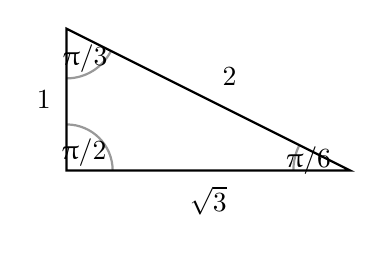
\begin{tikzpicture}[scale=0.9,thick]
\coordinate (O) at (0,0);
\coordinate (A) at (4,0);
\coordinate (B) at (0,2);
\draw (O)--(A)--(B)--cycle;

\tkzLabelSegment[below=2pt](O,A){$\sqrt{3}$}
\tkzLabelSegment[left=2pt](O,B){$1$}
\tkzLabelSegment[above right=2pt](A,B){2}

\tkzMarkAngle[fill= orange,size=0.65cm,%
opacity=.4](A,O,B)
\tkzLabelAngle[pos = 0.35](A,O,B){$\uppi/2$}

\tkzMarkAngle[fill= orange,size=0.8cm,%
opacity=.4](B,A,O)
\tkzLabelAngle[pos = 0.6](B,A,O){$\uppi/6$}

\tkzMarkAngle[fill= orange,size=0.7cm,%
opacity=.4](O,B,A)
\tkzLabelAngle[pos = 0.5](O,B,A){$\uppi/3$}



\end{tikzpicture}
\noindent \mbox{The 45-45-90 triangle} \\


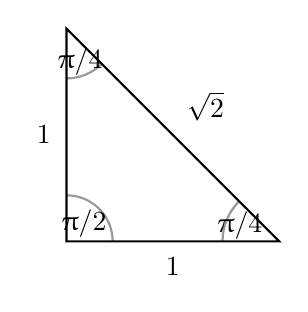
\begin{tikzpicture}[scale=0.9,thick]
\coordinate (O) at (0,0);
\coordinate (A) at (3,0);
\coordinate (B) at (0,3);
\draw (O)--(A)--(B)--cycle;

\tkzLabelSegment[below=2pt](O,A){$1$}
\tkzLabelSegment[left=2pt](O,B){$1$}
\tkzLabelSegment[above right=2pt](A,B){$\sqrt{2}$}
\tkzMarkAngle[fill= orange,size=0.65cm,%
opacity=.4](A,O,B)
\tkzLabelAngle[pos = 0.35](A,O,B){$\uppi/2$}

\tkzMarkAngle[fill= orange,size=0.8cm,%
opacity=.4](B,A,O)
\tkzLabelAngle[pos = 0.6](B,A,O){$\uppi/4$}

\tkzMarkAngle[fill= orange,size=0.7cm,%
opacity=.4](O,B,A)
\tkzLabelAngle[pos = 0.5](O,B,A){$\uppi/4$}
\end{tikzpicture}
\vspace{0.1in}
\section*{Laws of Cosine \& Sine}
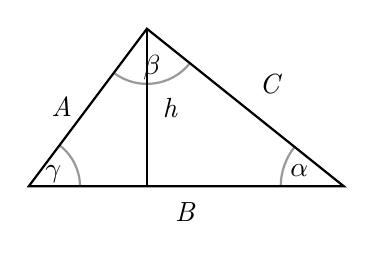
\begin{tikzpicture}[thick]
\coordinate (O) at (0,0);
\coordinate (A) at (4,0);
\coordinate (B) at (1.5,2);
\coordinate (C) at (1.5,0);
\draw (O)--(A)--(B)--cycle;
\draw (C)--(B)--cycle;

\tkzLabelSegment[below=2pt](O,A){\textit{B}}
\tkzLabelSegment[left=2pt](O,B){\textit{A}}
\tkzLabelSegment[above right=2pt](A,B){\textit{C}}
\tkzLabelSegment[right=2pt](C,B){\textit{h}}
\tkzMarkAngle[fill= orange,size=0.65cm,%
opacity=.4](A,O,B)
\tkzLabelAngle[pos = 0.35](A,O,B){$\gamma$}

\tkzMarkAngle[fill= orange,size=0.8cm,%
opacity=.4](B,A,O)
\tkzLabelAngle[pos = 0.6](B,A,O){$\alpha$}

\tkzMarkAngle[fill= orange,size=0.7cm,%
opacity=.4](O,B,A)
\tkzLabelAngle[pos = 0.5](O,B,A){$\beta$}
\end{tikzpicture}

\vspace{0.25in}

\noindent \textbf{Law of cosine:} \,
\(
    C^2 = A^2 + B^2 - 2 A B \cos(\gamma) 
\) \\

\noindent \textbf{Law of sines:} \,
\(
    \frac{\sin(\alpha)}{A} =  \frac{\sin(\beta)}{B} =  \frac{\sin(\gamma)}{C}
\) \\

\noindent \textbf{Area:} \,
\(
    \mbox{Area} = \nicefrac{1}{2} hB =   \nicefrac{1}{2} A B \sin(\gamma)
\)

\vspace{0.25in}
\section*{Volumes}

\noindent \textbf{Right Circular Cylinder} \\

\begin{minipage}[c]{0.25\textwidth}
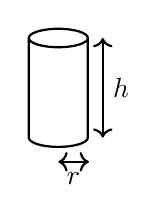
\begin{tikzpicture}[thick]
  \node (a) [cylinder, shape border rotate=90, draw, minimum height=15mm, minimum width=7.5mm] {};
  \draw [<->] ([xshift=5pt]a.before bottom) -- ([xshift=5pt]a.after top) node [midway, right] {$h$};
  \draw [<->] ([yshift=-5pt]a.bottom) -- ([yshift=-5pt]a.bottom -| a.before bottom) node [midway, below] {$r$};
\end{tikzpicture}
\end{minipage}
\begin{minipage}[l]{0.25\textwidth}
\noindent \textbf{Volume:} \,
\(
    \mbox{V} = \uppi r^2 h
\)

\noindent \textbf{Area:}  (not including circular ends)\,
\(
   \mbox{A} = 2 \uppi r  h
\)

\vspace{0.2in}
\noindent \textbf{Sphere} with radius $r$  \\

\noindent  \textbf{Area:}   \(A = 4 \uppi   r^2 \) \\
\noindent  \textbf{Volume:}   \(V = \frac{4 \uppi}{3} r^3 \)

\end{minipage}

\end{multicols*}

\begin{multicols*}{2}
\noindent \textbf{Cone} \\
  \begin{minipage}[c]{0.25\textwidth}
   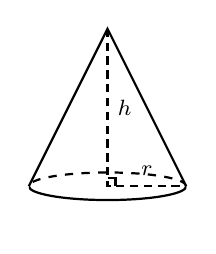
\begin{tikzpicture}[thick, scale=0.5]
      \begin{scope}
     \clip (-2,0) rectangle (2,1cm);
    \draw[dashed] (0,0) circle(2cm and 0.35cm);
    \end{scope}
    \begin{scope}
     \clip (-2,0) rectangle (2,-1cm);
    \draw (0,0) circle(2cm and 0.35cm);
    \end{scope}
    \draw[densely dashed] (0,4) -- node[right,font=\footnotesize] {$h$}coordinate[pos=0.95] (aa)(0,0)
                            -- node[above,font=\footnotesize] {$r$}coordinate[pos=0.1] (bb) (2,0);
    \draw (aa) -| (bb);
    \draw (-2,0) -- (0,4) -- (2,0);
  \end{tikzpicture}
  \end{minipage}
  \begin{minipage}[c]{0.25\textwidth}
  \noindent \textbf{Volume:} \,
  \(
     \mbox{V} = \nicefrac{\uppi r^2 h}{3}
  \) \\ 
  
\noindent \textbf{Area} \\
\(
   \mbox{A} =  \uppi r   \sqrt{r^2+h^2}
\)  (not including circular base).
\end{minipage}




\section*{P-Series, Divergence Test, Ratio Test, Comparison, \& AST}

\vspace{0.25in}
\begin{minipage}[c]{0.5\textwidth}
The series \(\sum_{k=1}^\infty \frac{1}{k^p}\) converges when $p \in (1,\infty)$;
otherwise it diverges.

%\vspace{0.25in}

If $\lim_{k \to \infty} a_k  \neq 0$, the series $\sum a_k$ diverges.

%\vspace{0.25in}

Let $a$ be a sequence with $0 \notin \range(a)$. Define 
$L = \lim_{k \to \infty} \left| \frac{a_{k+1}}{a_k} \right|$.
\begin{itemize}[noitemsep]
\item $L \in [0,1) \implies \sum |a_k| $ converges.
\item $L \in (1,\infty] \implies \sum a_k $ diverges.
\end{itemize}

%\vspace{0.25in} 

Let $a$ and $b$ be positive sequences. Define 
$L = \lim_{k \to \infty} \frac{a_k}{b_k}$.
\begin{itemize}[noitemsep]
    \item If $L \in \reals_{> 0}$ and $\sum a_k$ converges, then  
    $\sum b_k$ converges.

    \item If $L \in \reals_{> 0}$ and $\sum a_k$ diverges, then  
    $\sum b_k$ diverges.

    \item If $L = 0$ and $\sum b_k$  converges, then $\sum a_k $  converges
   
    \item If $L = \infty$ and $\sum b_k$ diverges, then $\sum a_k $ diverges.  
\end{itemize}

Let  $a$ be a positive and eventually decreasing sequence. 
Then $\sum (-1)^k a_k$ converges if and only if $\lim_{k \to \infty} a_k = 0$.

\end{minipage}



\vspace{0.125in}
\section*{Taylor and MacLaurin Series}
\vspace{0.25in}
If a function $F$ is infinitely differentiable at $a$, its Taylor series centered at $a$ is
\begin{equation*}
  \sum_{k=0}^\infty \frac{F^{(k)}(a)}{k!}  (x-a)^k.
\end{equation*}
When $a$ is zero, the Taylor series is also known as a MacLaurin Series.
\vspace{0.1in}
\section*{Polar to Cartesian}
%\vspace{-0.2in}
\begin{minipage}[c]{0.5\textwidth}
\begin{equation*}
x = r \cos(\theta) \quad y = r \sin(\theta)
\end{equation*}
For $r > 0$ and $0 \leq \theta < 2 \uppi$
\begin{equation*}
r = \sqrt{x^2 + y^2} ,\quad 
\theta = \begin{cases} 2 \uppi - \arccos(\nicefrac{x}{r})  & \mbox{ if } y < 0  \\
  \arccos(\nicefrac{x}{r})  & \mbox{ if } y \geq 0 
             \end{cases}    
\end{equation*}
\end{minipage}      

\section*{Integrate Powers of Trig}
\vspace{0.1in}
Let $m,n \in \integers_{\geq 0}$. Then

\begin{itemize}[noitemsep]
  \item $\int \cos(x)^{2m} \sin(x)^{2n} \, \mathrm{d}x
         = \int \left(\frac{1+\cos(2 x)}{2}\right)^m 
                 \left(\frac{1-\cos(2 x)}{2}\right)^n 
                 \, \mathrm{d}x$

  \item $\int \cos(x)^{2m+1} \sin(x)^{n} \, \mathrm{d}x
  = \int (1-z^2)^m  z^{n}
             \, \mathrm{d}z$,  where $z = \sin(x)$

  \item $\int \cos(x)^{m} \sin(x)^{2n+1} \, \mathrm{d}x
             = -\int z^m (1-z^2)^n \, \mathrm{d}z$,  
             where $z = \cos(x)$

\item $\int \sec(x)^n \, \mathrm{d} x = \frac{1}{n-1} \sec(x)^{n-2} \tan(x) + \frac{n-2}{n-1} \int \sec(x)^{n-2} \, \mathrm{d} x$,
provided $n \neq 1$.
\item $\int \tan(x)^{2m+1} \sec(x)^n \, \mathrm{d} x =  \int (z^2-1)^m z^{n-1} \, \mathrm{d} z$,
where $z=\sec(x)$

\item $\int \tan(x)^{2m} \sec(x)^n \, \mathrm{d} x  = \int (\sec(x)^2-1)^m \sec(x)^n \, \mathrm{d} x$.


\end{itemize}
              \vspace{0.050in}
\section*{Trig Substitutions}
\vspace{0.25in}
\begin{itemize}[noitemsep]
\item $\int F \left(x, \left(1-x^2\right)^{n/2}\right) \, \mathrm{d} x$, 
use $x = \sin(\vartheta)$, where  $\vartheta \in [-\uppi/2, \uppi/2]$
, then integrate $\int F \left(\sin(\vartheta),\cos(\vartheta)^n\right) \cos(\vartheta) \, \mathrm{d} \vartheta$
\item  $\int F\left(x, \left (1+x^2 \right)^{n/2}\right) \, 
\mathrm{d} x$, use $x = \sinh(\vartheta)$,
where $\vartheta \in \reals$, then integrate
$\int F\left(\sinh(\vartheta), \cosh(\vartheta)^n \right)  \cosh(\vartheta)\, \mathrm{d} \vartheta$

\item  $\int F \left(x, \left(x^2-1\right)^{n/2} \right) \, \mathrm{d} x$, 
use $x = \sec(\vartheta)$, then  integrate \\
$\int F(\sec(\vartheta), \tan(\vartheta)^n) \sec(\vartheta)\, \tan(\vartheta) 
\, \mathrm{d} \vartheta)$
\end{itemize}

\vspace{0.25in}
\section*{Unit Circle}

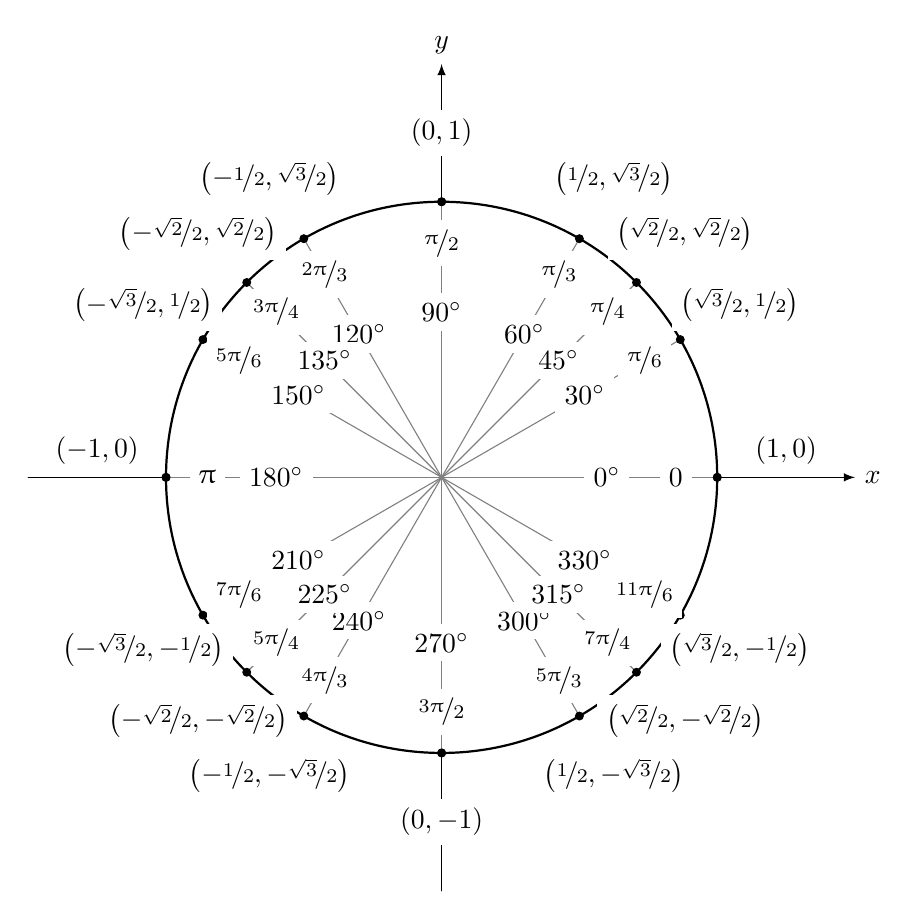
\begin{tikzpicture}[scale=3.5,cap=round,>=latex]
    % draw the coordinates
    \draw[->] (-1.5cm,0cm) -- (1.5cm,0cm) node[right,fill=white] {$x$};
    \draw[->] (0cm,-1.5cm) -- (0cm,1.5cm) node[above,fill=white] {$y$};

    % draw the unit circle
    \draw[thick] (0cm,0cm) circle(1cm);

    \foreach \x in {0,30,...,330} {
            % lines from center to point
            \draw[gray] (0cm,0cm) -- (\x:1cm);
            % dots at each point
            \filldraw[black] (\x:1cm) circle(0.4pt);
            % draw each angle in degrees
            \draw (\x:0.6cm) node[fill=white] {$\x^\circ$};
    }

    \foreach \x in {0,45,...,315} {
            % lines from center to point
            \draw[gray] (0cm,0cm) -- (\x:1cm);
            % dots at each point
            \filldraw[black] (\x:1cm) circle(0.4pt);
            % draw each angle in degrees
            \draw (\x:0.6cm) node[fill=white] {$\x^\circ$};
    }

    % draw each angle in radians
    \foreach \x/\xtext in {
        30/\nicefrac{\uppi}{6},
        45/\nicefrac{\uppi}{4},
        60/\nicefrac{\uppi}{3},
        90/\nicefrac{\uppi}{2},
        120/\nicefrac{2\uppi}{3},
        135/\nicefrac{3\uppi}{4},
        150/\nicefrac{5\uppi}{6},
        180/\uppi,
        210/\nicefrac{7\uppi}{6},
        225/\nicefrac{5\uppi}{4},
        240/\nicefrac{4\uppi}{3},
        270/\nicefrac{3\uppi}{2},
        300/\nicefrac{5\uppi}{3},
        315/\nicefrac{7\uppi}{4},
        330/\nicefrac{11\uppi}{6},
        0/0}
            \draw (\x:0.85cm) node[fill=white] {$\xtext$};

    \foreach \x/\xtext/\y in {
        % the coordinates for the first quadrant
        30/\nicefrac{\sqrt{3}}{2}/\nicefrac{1}{2},
        45/\nicefrac{\sqrt{2}}{2}/\nicefrac{\sqrt{2}}{2},
        60/\nicefrac{1}{2}/\nicefrac{\sqrt{3}}{2},
        % the coordinates for the second quadrant
        150/-\nicefrac{\sqrt{3}}{2}/\nicefrac{1}{2},
        135/-\nicefrac{\sqrt{2}}{2}/\nicefrac{\sqrt{2}}{2},
        120/-\nicefrac{1}{2}/\nicefrac{\sqrt{3}}{2},
        % the coordinates for the third quadrant
        210/-\nicefrac{\sqrt{3}}{2}/-\nicefrac{1}{2},
        225/-\nicefrac{\sqrt{2}}{2}/-\nicefrac{\sqrt{2}}{2},
        240/-\nicefrac{1}{2}/-\nicefrac{\sqrt{3}}{2},
        % the coordinates for the fourth quadrant
        330/\nicefrac{\sqrt{3}}{2}/-\nicefrac{1}{2},
        315/\nicefrac{\sqrt{2}}{2}/-\nicefrac{\sqrt{2}}{2},
        300/\nicefrac{1}{2}/-\nicefrac{\sqrt{3}}{2}}
            \draw (\x:1.25cm) node[fill=white] {$\left(\xtext,\y\right)$};

    % draw the horizontal and vertical coordinates
    % the placement is better this way
    \draw (-1.25cm,0cm) node[above=1pt] {$(-1,0)$}
          (1.25cm,0cm)  node[above=1pt] {$(1,0)$}
          (0cm,-1.25cm) node[fill=white] {$(0,-1)$}
          (0cm,1.25cm)  node[fill=white] {$(0,1)$};
\end{tikzpicture}

\vfill 
\noindent Revised \today. Barton Willis is the author of this work. This work is
licensed under Attribution 4.0 International (CC BY 4.0) \,  \qrcode[height=0.15in]{https://creativecommons.org/licenses/by/4.0/}. For the current version of
this document, visit \, \qrcode[height=0.15in]{https://github.com/barton-willis/calculus-two} 

\end{multicols*}
\end{document}

